% ----------------------------------------------------
% Literature Review
% ----------------------------------------------------

\chapter{Literature Review}\label{ch:literature}

\section{A Brief History of Salinity}\label{sec:a-brief-history-of-salinity}
The most common definition of salinity relates it to the total amount of dissolved \textit{salts} in a solution, however, salinity's definition has had several more complex iterations over the years.
The first definition of salinity was the total amount of dissolved \textit{material} in grams in one kilogram of water~\cite{stewart_introduction_to_physical_oceanography_2004}.
This is a dimensionless quantity was expressed in \gls{ppt} or $g.kg^{-1}$ where most ocean water's salinity falls between 34.60\gls{ppt} and 34.80\gls{ppt} as shown in \reffig{fig:ocean_salinity_temperature_quantity}.
\begin{figure}[h]
    \centering
    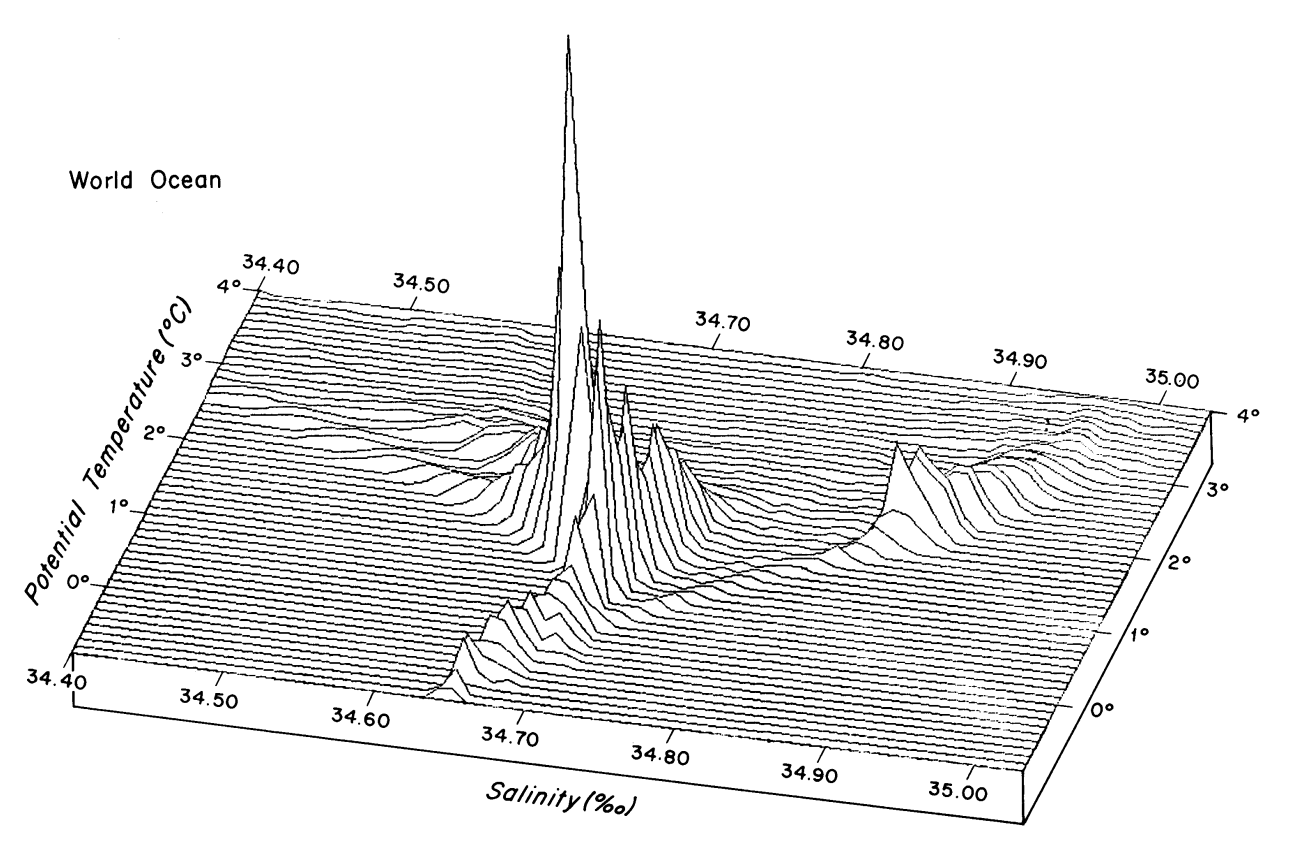
\includegraphics[width=0.75\textwidth]{Figures/ocean_salinity_temperature_quantity}
    \caption{Histogram showing the volume of ocean water relative to temperature and salinity bins. The highest peak corresponds to a volume of 26 million cubic kilometers of ocean water~\cite{worthington_ocean_graphs_1981}.}
    \label{fig:ocean_salinity_temperature_quantity} %chktex 24
\end{figure}
The probelm with this definition of salinity lay with its testibility.
Trying to obtain the mass of the dissolved material through evaporation removed certain compounds making this method almost impossible to achieve~\cite{sverdrup_ocean_physics_and_chemistry_1942} and thus salinity needed to be redefined in a way that was easily and reliably testable.
The next definition of salinity related it to the amount of chlorine present in the water, or the chlorinity of the water.
Thus, in 1969, salinity was redefined to be directly proportional to the chlorinity of the water~\cite{stewart_introduction_to_physical_oceanography_2004}.
The calculation of salinity from chlorinity is further discussed in~\refsec{subsec:the-salinity-chlorinity-relationship}.

Around the same time as the salinity-chlorinity relationship was established, oceanographers had begun experiementing with the use of conductivity to measure salinity.
Conductivity was found to be more precise and significantly easier to measure than the titration required to measure chlorinity~\cite{lewis_salinity_definition_and_calculation_1978}.
In 1978, the Practical Salinity Scale was established and salinity was updated to be related to conductivity which is the current defintion of salinity\cite{lewis_salinity_definition_and_calculation_1978}.
This relation also included terms for temperature and depth as these affect the conductivity of an electrolyte solution~\cite{zheng_electrical_conductivity_of_ocean_2017}.

The Practical Salinity Scale uses its own dimensionless units of salinity which are not interchangeable with \gls{ppt} in the current definition of salinity.
Although the Practical Salinity Scale is sometimes given in \gls{psu}, it is more technically correct to refer to it as a certain Practical Salinity `on the Practical Salinity Scale PSS-78'~\cite{lewis_salinity_definition_and_calculation_1978}.
The calculation of salinity from conductivity is further discussed in~\refsec{subsec:the-salinity-conductivity-relationship}.

% \section{The Uses of Salinity Measurements}\label{sec:the-uses-of-salinity-measurements}
% oceanography, speciation, conservation, habitation, water quality (drinking, agriculture, industrial), aquaculture, desalination.
% antarctic ice.

\section{Salinity Measurement Methods and Devices}\label{sec:salinity-measurement-techniques}

Salinity has had a long history of being measured using a variety of methods with varying degrees of accuracy.
Currently, the most common method of measuring salinity is through the use of a \gls{ctd} which is a device that measures the conductivity, temperature, and depth of a sample of water.
\textit{table summary}

\subsection{Salinity from Chlorinity}\label{subsec:salinity-from-chlorinity}

The chemical composition of ocean water with a salinity of 35\gls{ppt} contains 19.35\gls{ppt} of Chlorine and 10.77\gls{ppt} of Sodium with the following ions only accounting for a total of just above 3\gls{ppt} of the total dissolved solids in the water~\cite{britannica_seawater_encyclopaedia_2024}.
This allowed oceanographers to estimate that the salinity of ocean water was directly proportional to the amount of chlorine in the water.
The chlorinity of a solution had an established definition which was `the mass of silver required to precipitatecompletely the halogens in $0.328\ 523\ 4 kg$ of the ocean-water sample'~\cite{wooster_redefinition_of_salinity_1969} which could be tested to a degree of accuracy using titration.
In 1969, an accurate relationship between these was established by~\refref{wooster_redefinition_of_salinity_1969} and thus salinity $S$ was redefined using chlorinity $Cl$ as shown in~\refeqn{eq:salinity-chlorinity}.
\begin{equation}\label{eq:salinity-chlorinity}
    S (\text{\gls{ppt}}) = 1.80655 \times~Cl (\text{\gls{ppt}})
\end{equation}
\textit{accuracy achieved?, device?, limitations?}

\subsection{Salinity from Conductivity}\label{subsec:salinity-from-conductivity}

\subsection{Salinity from Density}

\subsection{Salinity from Microwaves}

\subsection{Salinity from Satellite Remote Sensing}

\subsection{Salinity from Interferometry}

\subsection{Salinity from Electromagnetic Induction}

\subsection{Salinity from Refractive Index}

\section{Salinity Measurement Devices}\label{sec:salinity-measurement-devices}
CTDs, refractometers, conductivity meters, salinometers.

% ----------------------------------------------------
% Theory Development
% ----------------------------------------------------

\chapter{Theory Development}\label{ch:theory-development}

\section{The Calculation of Salinity}\label{sec:the-calculation-of-salinity}

\subsection{The Salinity and Chlorinity Relationship}\label{subsec:the-salinity-chlorinity-relationship}

\subsection{The Salinity and Conductivity Relationship}\label{subsec:the-salinity-conductivity-relationship}

Salinity meters that use electrical conductivity are commonly known as \gls{ctd}s which stands for \gls{ctd}.
As depth is a measurement derived from pressure, CTp is the prefered designation when performing calculations.
This allows for the conductivity of a sample of water to be denoted by $C(S, T, p)$ where conductivity is a functon of salinity $S$, temperature $T$, and pressure $p$ which is the convention in oceanography~\cite{lewis_salinity_definition_and_calculation_1978}.

Pressure in the salinity equation is taken relative to sea level where $p = 0 dbar$ is equivalent to an absolute pressure of $P = 101\ 325 Pa$.
Using decibars (dbar) for pressure is a common practice in oceanography as it is a unit of pressure that is equal to roughly one meter of water depth~\cite{seabird_dbar_to_depth_2024}.

The Practical Salinity Scale defines Practical salinity $S_p$ in terms of a conductivity ratio $K_{15}$ which is the conductivity of a sample of water at a temperature of $15\degree C$ and a pressure equal to one standard atmosphere divided by the conductivity of a standard potassium chloride solution at the same temperature and pressure.
The standard potassium chloride solution is $32.4356g$ of $KCl$ dissolved in $1.000kg$ of water and when the ratio between the conductivity of a sample of water and the standard solution, or $K_{15}$, equals 1 the Practical Salinity $S_p$ is, by definition, 35.

When $K_{15}$ is not equal to 1, the Practical Salinity $S_p$ can be calculated using the PSS-78 equation shown in \refeqn{eq:pss-78-k15}.
\begin{equation}\label{eq:pss-78-k15}
    S_p = \sum_{i=0}^{5} a_i {(K_{15})}^{i/2}~~~~\text{where}~~~~K_{15} = \frac{C(S_p, 15\degree C, 0)}{C(35, 15\degree C, 0)}
\end{equation}
All the coefficients for the salinity-conductivity equations, including $a_i$, are given in~\reftab{tab:pss-78-coefficients}.

To calculate the salinity of a sample of water that is not at $15\degree C$ and $0 dbar$, the conductivity ratio of the sample can be expanded into the product of three ratios which are labelled $R_p$, $R_t$, and $r_t$ respectively.
The conductivity measurement taken in the field $C(S_p, t, p)$ is related to the conductivity of the standard solution $C(S_p, 15\degree C, 0)$ which the device is calibrated with and is represented by $R$ in \refeqn{eq:pss-78-full-ratio}.~\cite{ioc_teos_2010}
\begin{equation}\label{eq:pss-78-full-ratio}
    R = \lfrac{C(S_p, t, p)}{C(S_p, 15\degree C, 0)} = \lfrac{C(S_p, t, p)}{C(S_p, t, 0)} \cdot \lfrac{C(S_p, t, 0)}{C(35, t, 0)} \cdot \lfrac{C(35, t, 0)}{C(35, 15\degree C, 0)} = R_p R_t r_t
\end{equation}
In order the calculate the salinity of the sample $R_t$ must be found which takes a similar for to $K_{15}$.
$r_t$ is first calculated using the temperature of the sample 
\begin{equation}\label{eq:pss-78-rt}
    r_t = \sum_{i=0}^{4} c_i {(t)}^i
\end{equation}
following which $R_p$ is calculated using the sample's pressure $p$, temperature $t$ and conductivity ratio $R$,
\begin{equation}\label{eq:pss-78-rp}
    R_p = 1 + \lfrac{\sum_{i=1}^{3} e_i p^i}{1 + d_1 (t) + d_2 {(t)}^2 + R\left[ d_3 + d_4 (t) \right]}
\end{equation}
and finally $R_t$ is calculated using $r_t$, $R_p$ and $R$.
\begin{equation}\label{eq:pss-78-Rt}
    R_t = \lfrac{R}{R_p r_t}
\end{equation}
Note that for a sample temperature of $15\degree C$ and pressure of $0 dbar$, $r_t$ and $R_t$ both equal 1 which leaves $R_t$ equal to $R$ and thus \refeqn{eq:pss-78-k15} can be used to calculate the Practical Salinity $S_p$.
For temperatures other than $15\degree C$, the Practical Salinity $S_p$ can be calculated using \refeqn{eq:pss-78-full} where $k = 0.0162$.~\cite{ioc_teos_2010}
\begin{equation}\label{eq:pss-78-full}
    S_p = \sum_{i=0}^{5} a_i {(R_t)}^{i/2} + \lfrac{t-15}{1+k(t-15)} \sum_{i=0}^{5} b_i {(R_t)}^{i/2}
\end{equation}

% chktex-file 44    
\begin{longtblr}[
    caption = {Coefficients for the PSS-78 equations~\cite{ioc_teos_2010}.},
    label = {tab:pss-78-coefficients}
    ]{
    colspec = {|q{1.5cm}|C|C|C|C|C|}
    }
    \hline
    \textbf{$i$} & \textbf{$a_i$} & \textbf{$b_i$} & \textbf{$c_i$} & \textbf{$d_i$} & \textbf{$e_i$} \\
    \hline
    $0$ & $0.0080$ & $0.0005$ & $6.766097\e{-1}$ & & \\
    \hline
    $1$ & $-0.1692$ & $-0.0056$ & $2.00564\e{-2}$ & $3.426\e{-2}$ & $2.070\e{-5}$ \\
    \hline
    $2$ & $25.3851$ & $-0.0066$ & $1.104259\e{-4}$ & $4.464\e{-4}$ & $-6.370\e{-10}$ \\
    \hline
    $3$ & $14.0941$ & $-0.0375$ & $-6.9698\e{-7}$ & $-4.215\e{-3}$ & $3.989\e{-15}$ \\
    \hline
    $4$ & $-7.0261$ & $0.0636$ & $1.0031\e{-9}$ & $-3.107\e{-3}$ & \\
    \hline
    $5$ & $2.7081$ & $-0.0144$ & & & \\
    \hline
\end{longtblr}
Note that the coefficients $a_i$ precisely sum to 35 such that the Practical Salinity $S_p$ is 35 when $K_{15}$ or $R_t = 1$ as per \refeqn{eq:pss-78-k15} and \refeqn{eq:pss-78-full}.
Additionally, the coefficients $b_i$ precisely sum to 0 such that the Practical Salinity $S_p$ does not depend on the temperature of the water when $R_t = 1$ as per \refeqn{eq:pss-78-full}.~\cite{ioc_teos_2010}

\refeqn{eq:pss-78-k15} to \refeqn{eq:pss-78-full} are valid for $2 < S_p < 42$ and $-2\degree C < t < 35\degree C$ and $0 dbar < p < 10\ 000 dbar$~\cite{ioc_teos_2010}.
The range for salinity has been extended using estimations by \refref{hill_extension_of_pss_low_1986} for $0 < S_p < 2$ and \refref{poisson_extension_of_pss_high_1993} for $42 < S_p < 50$.

The temperatures used in \refeqn{eq:pss-78-k15} to \refeqn{eq:pss-78-full} are on the IPTS-68 scale~\cite{furukawa_ipts68_1973} and have not been corrected to the currently used ITS-90 scale~\cite{preston_its90_1990}. 
In order to correctly calculate the salinity, the temperatures should be converted to the IPTS-68 scale using the equation $t_{68} = 1.00024 t_{90}$ before calculating salinity~\cite{preston_its90_1990}.

\section{Electrical Characteristics of Salt Water}\label{sec:electrical-characteristics-of-salt-water}
PSU vs TSD vs conductivity vs resistivity, salinity equation, capacitance of salt water, non-constant conductivity vs voltage.

\section{External Factors Affecting Electrical Characteristics of Salt Water}\label{sec:external-factors-affecting-electrical-characteristics-of-salt-water}

\section{Electrical Fringing in Concductive Materials}

\section{Electromagnetic Interference of Salt Water}

% ----------------------------------------------------
%current CTDs
%
%electrical conductivity sensor https://link.springer.com/article/10.1007/s11270-020-04971-7
%
%arduino version https://www.instructables.com/Water-Salinity-meter/
%
%mini version https://www.diva-portal.org/smash/get/diva2:512332/FULLTEXT01.pdf
%
%% ----------------------------------------------------
%measurement techniques
%
%high res https://link.springer.com/chapter/10.1007/978-1-4615-9182-5_18
%
%salinity and its measurands https://iopscience.iop.org/article/10.1088/1681-7575/aaea92/pdf
%
%interferometer https://iopscience.iop.org/article/10.1088/0957-0233/20/3/034003/meta?casa_token=ZTZbYNUpO0kAAAAA:7jvq44f2kE5qGGEQWt5ji18A7xWG4p9ZT4Ny99eOjMPOfywPIgqRNoCeH0VZby1VjlART_v77WV3rxfwi0k1nwphxfguYA
%
%the whole suite, important for later https://www.researchgate.net/profile/Bjoern-Kjerfve/publication/255660361_Measurement_and_Analysis_of_Water_Current_Temperature_Salinity_and_Density/links/0c9605373c5d3088b4000000/Measurement-and-Analysis-of-Water-Current-Temperature-Salinity-and-Density.pdf
%
%microwave frequency https://www.sensorsportal.com/HTML/DIGEST/january_2014/Vol_162/P_1772.pdf
%
%refraction of light https://www.sciencedirect.com/science/article/abs/pii/S0925400503002922?casa_token=UDq5jm83UIsAAAAA:-UuQMhyBg9tuzleSc8tQnL2vuCv_HYHCB5AicHCTlBkBz_5gipNnDoA6DdPgBL9csU_wWS9lG6Bc
%
%conductivity using electromagnetism https://ieeexplore.ieee.org/abstract/document/7769877
%
%salinity equation paper https://agupubs.onlinelibrary.wiley.com/doi/abs/10.1029/jc083ic01p00466?casa_token=Om_oxKhUgLIAAAAA%3As_ZdT6Qn-zv9SSyC8G3io5r_0mxuepRxFE33jcaLtTNY4tyOQOLAObVtsjeQZ0gPpokwsmrEOP0pPHULQg
%
%% ----------------------------------------------------
%salinity properties
%
%temperature vs salinity https://link.springer.com/article/10.1023/B:EMAS.0000031719.83065.68
%
%salinity and other properties https://pubs.acs.org/doi/10.1021/es402188r
%
%salinity and it antecedents https://ieeexplore.ieee.org/stamp/stamp.jsp?tp=&arnumber=1145448
%
%salinity textbook https://pubs.acs.org/doi/pdf/10.1021/ja02205a013?casa_token=QPyPLh22vacAAAAA:O6Hc1M5FQEDZpJb4oUrGYzboIy0wWn__w6MxXGc8Aw7doPE9tz71yRCbmUtRSP5lOMdTr28U8bYI43IsBg
%
%electrical properties of salt ice https://pubs.acs.org/doi/full/10.1021/jp8055366?casa_token=qvssn_P9p_8AAAAA%3A1FY_4CW5oX_4P9gDNZfp0AaeByCkTF_WOcZ_hLbv2Y2FYsIRsO7ZZkqxzTHTo_MK4vWqfaqqQh2LagyDLA
%
%pressure and temperature increase conductivity https://journals.aps.org/pr/abstract/10.1103/PhysRev.70.329
%
%conductivity vs total dissolved solids https://iopscience.iop.org/article/10.1088/1755-1315/118/1/012019/meta
%
%% ----------------------------------------------------
%producers or CTDs
%
%https://www.whoi.edu/what-we-do/explore/instruments/instruments-sensors-samplers/conductivity-temperature-depth-ctd-sensors/
%
%% ----------------------------------------------------

